%% %% %% %%
%%
%% Parte C de la práctica
%%
%% %% %% %%

\documentclass[../procedimientos.tex]{subfiles}
\graphicspath{{\subfix{../../images/}}}

\begin{document}
\clearpage
\subsection{Parte C}
\subsubsection{Propuesta}
Se desea implementar un sistema que convierta un número en base 2 de cuatro 
bits a su representación en \textit{Código Grey} y otro sistema que haga el 
proceso inverso. De forma general, se tiene que un número $abcd_{(2)}$ tiene 
una representación $wxyz_{Grey}$ dada por la siguiente tabla:
\begin{table}[H]
  \centering
  \begin{tabular}{c|cccc|cccc}
    \hline
    HEX & a	& b	& c	& d	& w	& x	& y	& z\\
    \hline
    0	& 0	& 0	& 0	& 0	& 0	& 0	& 0	& 0\\
    1	& 0	& 0	& 0	& 1	& 0	& 0	& 0	& 1\\
    2	& 0	& 0	& 1	& 0	& 0	& 0	& 1	& 1\\
    3	& 0	& 0	& 1	& 1	& 0	& 0	& 1	& 0\\
    4	& 0	& 1	& 0	& 0	& 0	& 1	& 1	& 0\\
    5	& 0	& 1	& 0	& 1	& 0	& 1	& 1	& 1\\
    6	& 0	& 1	& 1	& 0	& 0	& 1	& 0	& 1\\
    7	& 0	& 1	& 1	& 1	& 0	& 1	& 0	& 0\\
    8	& 1	& 0	& 0	& 0	& 1	& 1	& 0	& 0\\
    9	& 1	& 0	& 0	& 1	& 1	& 1	& 0	& 1\\
    A	& 1	& 0	& 1	& 0	& 1	& 1	& 1	& 1\\
    B	& 1	& 0	& 1	& 1	& 1	& 1	& 1	& 0\\
    C	& 1	& 1	& 0	& 0	& 1	& 0	& 1	& 0\\
    D	& 1	& 1	& 0	& 1	& 1	& 0	& 1	& 1\\
    E	& 1	& 1	& 1	& 0	& 1	& 0	& 0	& 1\\
    F	& 1	& 1	& 1	& 1	& 1	& 0	& 0	& 0\\
    \hline
  \end{tabular}
  \caption{Relación entre Base 2 y Código Grey}
  \label{tab:bin_to_grey}
\end{table}

\subsubsection{Análisis}
Por la forma en la que trabaja el \textit{Código Grey}, se tiene el siguiente 
comportamiento:
\begin{itemize}
  \item $w(abcd) = a$
  \item $x(abcd) = a \oplus b$
  \item $y(abcd) = b \oplus c$
  \item $z(abcd) = c \oplus d$
\end{itemize}

Y por otra parte, se tiene que:
\begin{itemize}
  \item $a(wxyz) = w$
  \item $b(wxyz) = x \oplus a(wxyz)$
  \item $c(wxyz) = y \oplus b(wxyz)$
  \item $d(wxyz) = z \oplus c(wxyz)$
\end{itemize}

Lo interesante de este útimo conjunto de relaciones es que su definición es 
recurrente, es decir, $a(wxyz)$, $b(wxyz)$ y $c(wxyz)$ se comportan como 
salidas, pero a su vez también son entradas para calcular las sigueintes 
cifras.

\subsubsection{Implementación en Quartus}
Se crearon dos símbolos, uno para convertir de \textit{Base 2} a 
\textit{Código Grey} ($f_1$), y otro para convertir de \textit{Código Grey} a 
\textit{Base 2} ($f_2$). Las implementaciones se muestran a continuación:
\begin{figure}[H]
  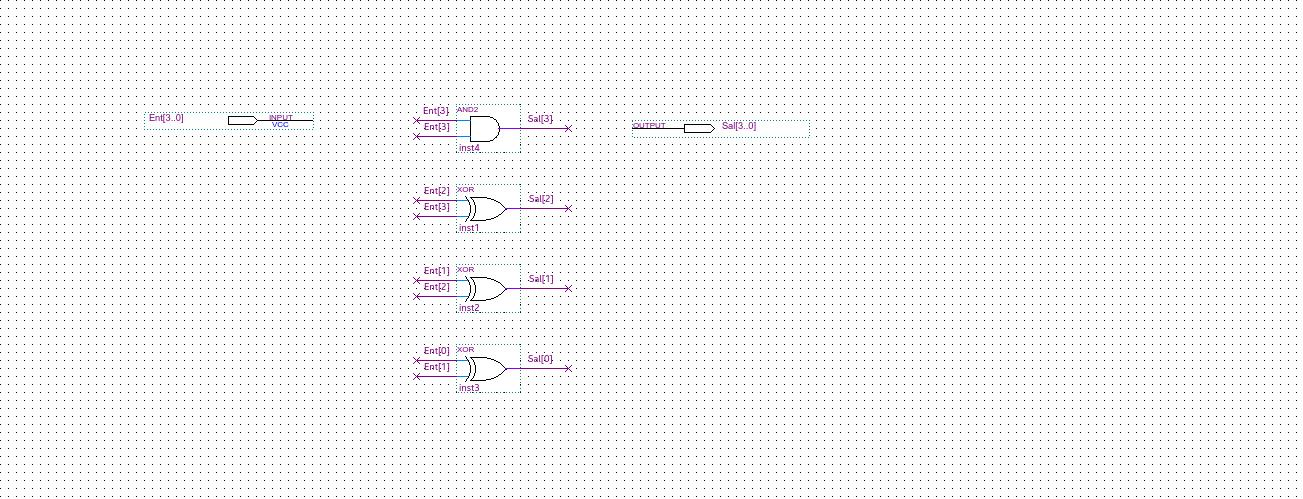
\includegraphics[width=\textwidth]{ejercicio_c1}
  \caption{Implementación de $f_1(abcd)$ (Parte C)}
  \label{fig:c_f1}
\end{figure}
\begin{figure}[H]
  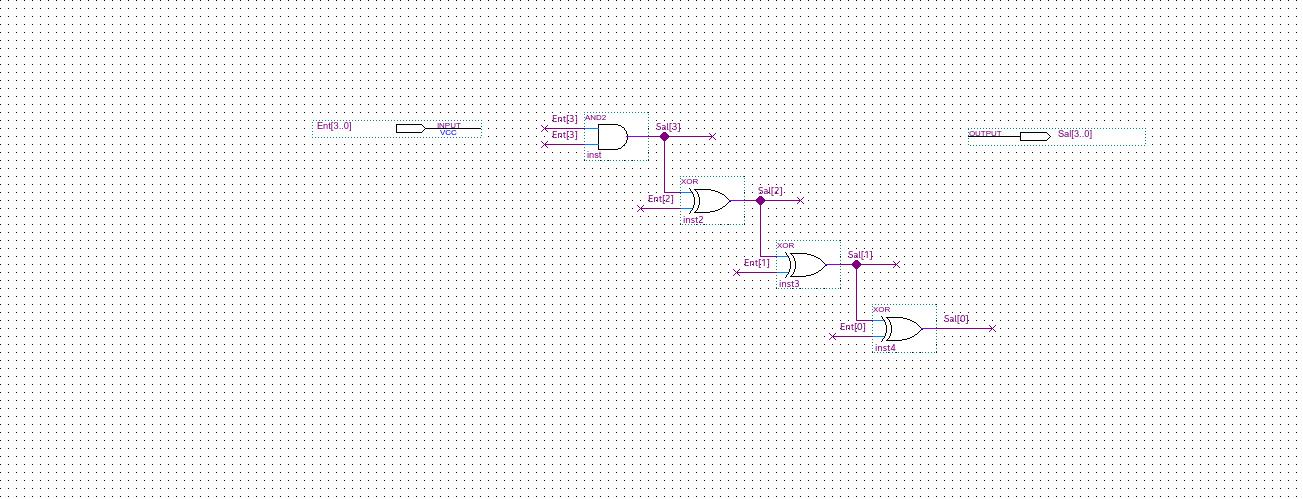
\includegraphics[width=\textwidth]{ejercicio_c2}
  \caption{Implementación de $f_2(wxyz)$ (Parte C)}
  \label{fig:c_f2}
\end{figure}

De forma general, cada uno de estos módulos ocupa etiquetas en los cables para 
reducir el número de conexiones físicas y así evitar errores; y arreglos para 
simplificar las entradas y las salidas. Ambos módulos se probaron de la 
siguiente forma:
\begin{figure}[H]
  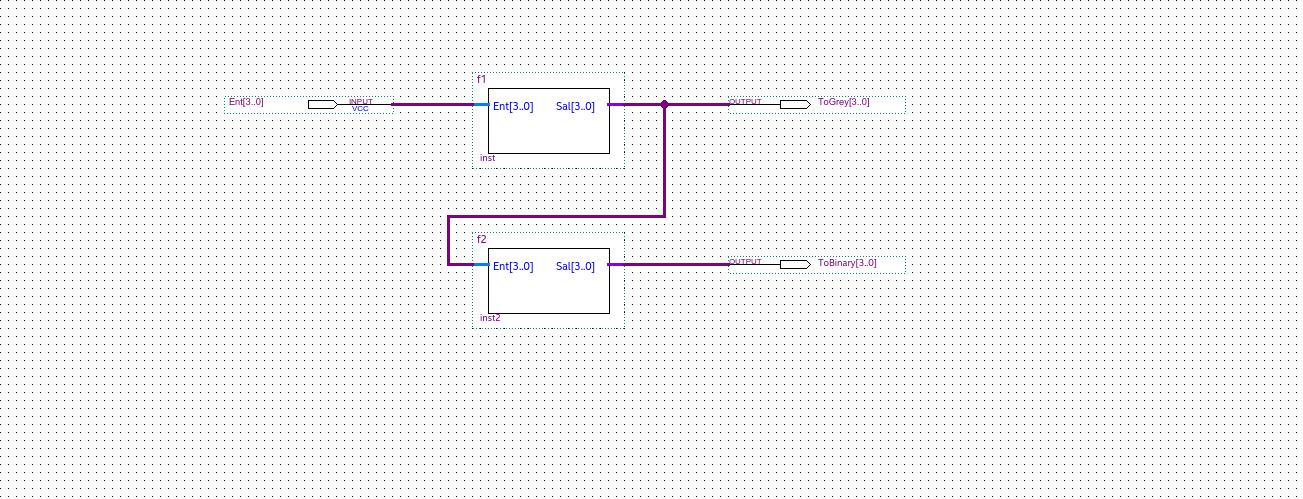
\includegraphics[width=\textwidth]{ejercicio_c}
  \caption{Implementación de la solución (Parte C)}
  \label{fig:c_complete}
\end{figure}

El sistema tiene una entrada en forma de arreglo (representación en bits del 
número binario a convertir) y dos salidas (una en \textit{Código Grey} y otra 
en \textit{Base 2}). Lo que se pretende es obtener la representación en 
\textit{Grey} (primera señal de salida) a través de $f_1(abcd)$ y 
posteriormente esa misma salida pasarla a $f_2(wxyz)$ para volver a obtener la 
misma señal de entrada.  Si lo anterior sucede, entonces los sistemas 
implementados funcionarán correctamente.

La comprobación de ambos sistemas se llevó a cabo a través de un 
\textit{diagrama de tiempos}, para el cual se configuró un archivo 
\textit{University Program VWF}. Ls imulación resultó en lo siguiente:
\begin{figure}[H]
  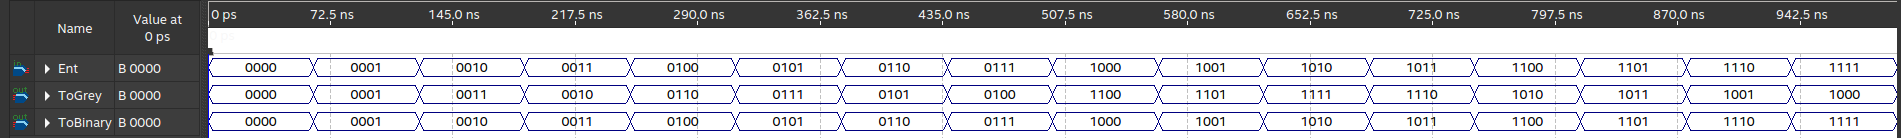
\includegraphics[width=\textwidth]{ejercicio_c_sim}
  \caption{Simulación (Parte A)}
  \label{fig:c_sim}
\end{figure}

Los resultados mostrados en la Figura \ref{fig:c_sim} son los mismos que se 
describen en la Tabla \ref{tab:bin_to_grey}. Además, la señal $Ent$ conicide 
de forma exacta con la señal $ToBin$. Esto indica que están bien implementados 
ambos sitemas.

\end{document}

